\documentclass[a4paper]{standalone}

% use this declaration to set specific page margins
%\usepackage[a4paper , lmargin = {2.7cm} , rmargin = {2.9cm} , tmargin = {2.7cm} , bmargin = {4.6cm} ]{geometry}
\usepackage[a4paper]{geometry}
\usepackage[ngerman, english]{babel}

\usepackage[utf8]{inputenc}
\usepackage[boxed]{algorithm2e}
\usepackage{amsmath}
\usepackage{amssymb}
\usepackage{authblk}
\usepackage{caption}
\usepackage{cleveref}
\usepackage [autostyle, english = american]{csquotes}
\usepackage{fontenc}
\usepackage{fontspec}
\usepackage{graphicx}
\usepackage[pagebackref=true]{hyperref}
\usepackage{multirow}
\usepackage[section]{placeins}
\usepackage{refstyle}
\usepackage{standalone}
\usepackage{subcaption}
\usepackage{tabularx}
\usepackage{url}
\usepackage{scrpage2}					% header and footer line


% header and footer line - no header & footer line on pages where a new chapter starts
\pagestyle{scrheadings}
\ohead{Mixing Text and Image Modalities in Artificial Neural Networks}
\ihead{Mario Tambos}
\ofoot[]{\thepage}
\ifoot{Master's Thesis, Mario Tambos, TU Berlin, Fachgebiet NI, 2018}

\MakeOuterQuote{"}

\newref{part}{name=part~,Name=Part~,names=parts~,Names=Parts~}
\newref{alg}{name=algorithm~,Name=Algorithm~,names=algorithms~,Names=Algorithms~}
\newref{sec}{name=section~,Name=Section~,names=sections~,Names=Sections~}
\newref{subsec}{name=subsection~,Name=Subsection~,names=subsections~,Names=Subsections~}

\newcommand{\vect}[1]{\mathbf{#1}}

\newcommand{\vecx}{\vect{x}}
\newcommand{\Dcal}{\mathcal{D}}
\newcommand{\Sbf}{\Sigma}
\newcommand{\Sbfs}{\Sigma^\star}
\newcommand{\Rbb}{\mathbb{R}}
\newcommand{\Nbb}{\mathbb{N}}

\makeatletter
\setlength{\@fptop}{0pt}
\makeatother

\makeatletter
\AtBeginDocument{%
    \expandafter\renewcommand\expandafter\subsection\expandafter{%
        \expandafter\@fb@secFB\subsection
    }%
}
\makeatother


\begin{document}
\section{Zero-shot learning}\label{sec:ZeroShotLearning}

In this final experiment we evaluate the performance of our method on a zero-shot learning task. Given a training set $\mathcal{D}^{(trn)}_N=\{(\vecx_i, y_i): \vecx_i \in \mathbf{X}, y_i \in \mathbf{Y}\}$ of N training pairs $(\vecx_i, y_i)$ and a model $\mathcal{M}$ trained on $\mathcal{D}^{(trn)}_N$, we want to evaluate $\mathcal{M}$ on a test dataset $\mathcal{D}^{(tst)}_M=\{(\vecx_j, \hat{y}_j): \vecx_j \in \mathbf{X}, \hat{y}_j \in \hat{\mathbf{Y}}\}$ of M test pairs $(\vecx_j, \hat{y}_j)$ with $\mathbf{Y} \neq \hat{\mathbf{Y}}$. It could be the case that $\mathbf{Y} \subsetneq \hat{\mathbf{Y}}$ or even $\mathbf{Y} \cap \hat{\mathbf{Y}} = \emptyset$.

In order to perform this experiment, and following Frome et al. \cite{frome2013devise}, we used three different datasets:
\begin{itemize}
%    \item ImageNet1K \cite{ILSVRC15}: is the dataset used in \secref{ImageClassification}.
    \item ImageNet21K \cite{ILSVRC15}: consists of 14,197,087 images divided into 21,841 different object classes.
    \item ImageNet1K - 2 Hops: was built by all images and classes in ImageNet21K, whose classes were at most 2 hops away in the WordNet \cite{miller1998wordnet} hierarchy from a class in ImageNet1K, the dataset used in \secref{ImageClassification}.
    \item ImageNet1K - 3 Hops: was built by all images and classes in ImageNet21K, whose classes were at most 3 hops away in the WordNet  hierarchy from a class in ImageNet1K.
\end{itemize}

Also like Frome et al. \cite{frome2013devise}, we used both the "flat hit @ k" employed \secref{ImageClassification}, as well as their "hierarchical hit @ k", defined as:

\begin{small}
    $$
        hierarchical\ hit @ k = \frac{1}{N}\sum_{N}^{i=1}\frac{\text{\# of model's top } k \text{ predictions} \in CorrectSet(trueLabel_i)}{k}\label{eq:h_at_k}\qquad (4.3)
    $$
\end{small}

where $CorrectSet(trueLabel_i)$ is created for each label in a test dataset as shown in \algref{CreateCorrectSet}, and $trueLabel_i$ is the true label corresponding to the $i$th image.
By reporting "hierarchical hit @ k" we try to take into account semantic similarities among the class labels: synonymy, hypernymy ("canine" is a hypernym of "dog"), coordinate terms ("wolf" is a coordinate term of "dog", and vice-versa), etc. Then, if our model predicted "pen" for an image with true label "pencil", "flat hit @ k" would be 0, but there is some $CorrectSet$ for which "hierarchical hit @ k" will be non-zero.

\begin{algorithm}[h]
    \SetKwFunction{CreateCorrectSet}{CreateCorrectSet}
    \CreateCorrectSet{$trueLabel$, $k$, $validLabels$}\\
    \KwData{
        
        $trueLabel$: class label in a test dataset.\\
        $k$: Minimum size of the $CorrectSet$.\\
        $validLabels$: set of labels allowed as members of $CorrectSet$.
    }
    \KwResult{$CorrectSet(trueLabel)$: equivalence set of labels for $trueLabel$}
    \Begin{
        $R \gets 0$\;
        \While{$|CorrectSet| < k$}{
            $radiusSet \gets $ all members of $validLabels$ that are $R$ hops from $trueLabel$ in the WordNet hierarchy.\;
            $CorrectSet \gets CorrectSet \cup radiusSet$\;
            $R \gets R + 1$\;
        }
    }
    \caption{$CorrectSet$ creation procedure, defined in \cite{frome2013devise}}\label{alg:CreateCorrectSet}
\end{algorithm}


The number of unique classes in the test datasets used for the zero-shot experiments, together with the mean sizes of the corresponding $CorrectSet$s at $k$, are shown in \figref{ZeroShotDatasetClassesNr} and \tabref{ZeroShotDatasetClassesNr}. In some cases, these numbers are extremely different from the ones reported by Frome et al.. Consequently, we decided not to include their results for comparison, as the methods we used for creating our test sets and calculating our performance metrics might not be comparable with theirs. Instead, we decided to use a random classifier as a baseline.

\begin{figure}[ht]
    \centering
    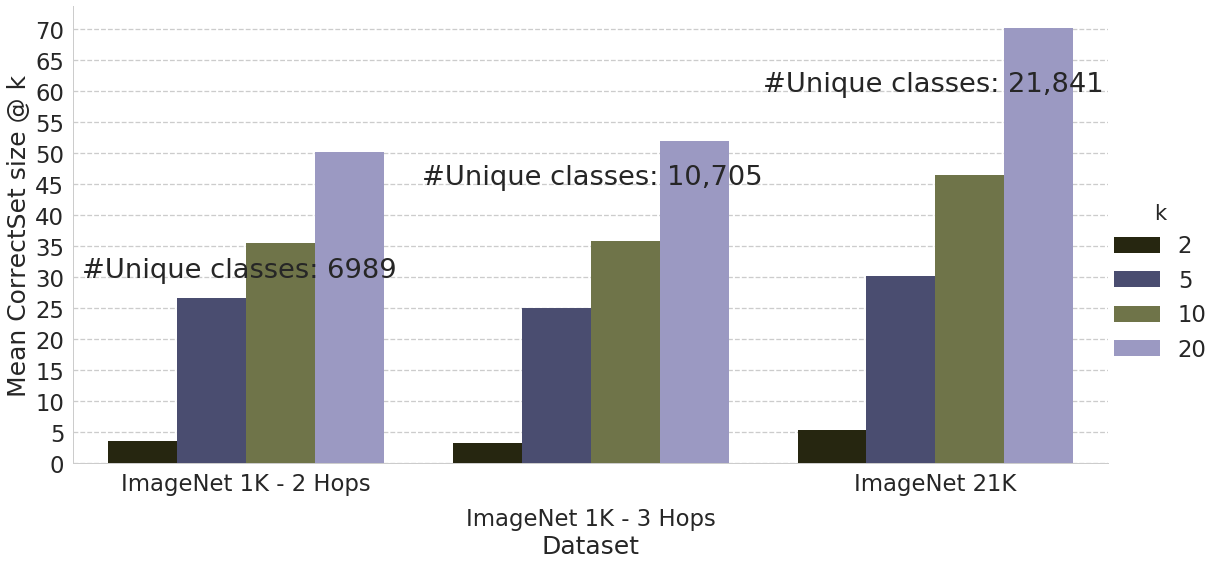
\includegraphics[width=\textwidth]{images/zero_shot_data_info.png}
    \caption{Number of unique classes in the test datasets used for the zero-shot experiments, together with the mean sizes of the corresponding $CorrectSet$s at $k$.}
    \label{fig:ZeroShotDatasetClassesNr}
\end{figure}

\begin{table}[h]
    \centering
    \begin{footnotesize}
        \begin{tabularx}{\textwidth}{|X|c|c|c|c|c|}
            \hline
            \multirow{2}{*}{Dataset} & \multirow{2}{*}{\# Unique classes} & \multicolumn{4}{c|}{Mean $CorrectSet$ size @ k} \\
            \cline{3-6}              &                                    & k=2      & k=5      & k=10     & k=20           \\ 
            \hline
%            ImageNet1K               & 1000                               & 3.062    & 16.031   & 25.413   & 41.583         \\ 
            ImageNet1K - 2 Hops      & 6989                               & 3.587    & 26.586   & 35.472   & 50.122         \\ 
            ImageNet1K - 3 Hops      & 10,705                             & 3.320    & 24.992   & 35.824   & 52.001         \\ 
            ImageNet21K              & 21,841                             & 5.350    & 30.160   & 46.517   & 70.111         \\ 
            \hline
        \end{tabularx}
    \end{footnotesize}
    \caption{Number of unique classes in the test datasets used for the zero-shot experiments, together with the mean sizes of the corresponding $CorrectSet$s at $k$.}
    \label{tab:ZeroShotDatasetClassesNr}
\end{table}


To execute the experiments in this section we employed the same \verb|MMSOM-W2V-CNN| model trained in \secref{ImageClassification}. However, in this case we did not work with the NN Classifier built into \verb|MMSOM-W2V-CNN|, but rather operated directly with the internal SOM model. Our predictions rely entirely on \algref{RetrieveWord}. The results we have obtained are shown in \tabref{ZeroShotFlatResults, ZeroShotHierarchicalResults} for the "flat hit @ k" and "hierarchical hit @ k" metrics, respectively.

\begin{figure}[h]
    \centering
    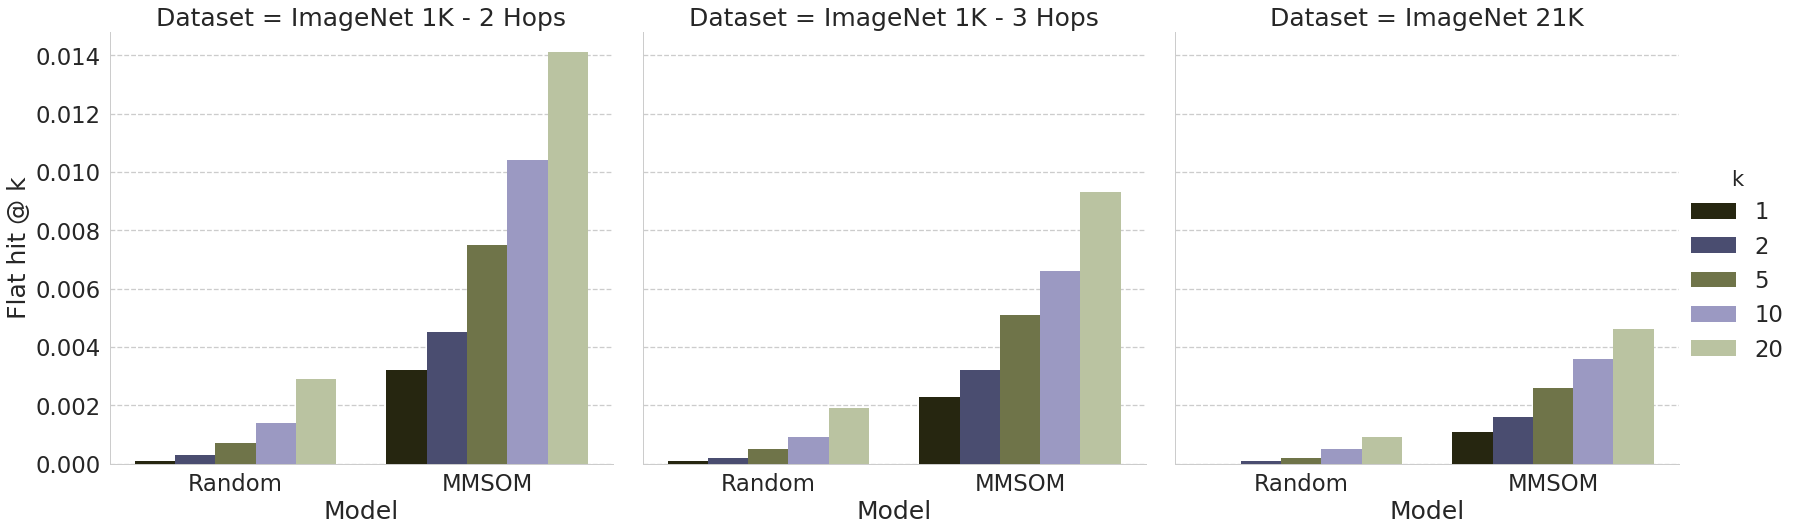
\includegraphics[width=\textwidth]{images/zero_shot_flat_results.png}
    \caption{Zero-shot learning experiment - "flat hit @ k" metric.}
    \label{figZeroShotFlatResults}
\end{figure}

\begin{table}[h]
    \centering
    \begin{footnotesize}
        \begin{tabularx}{\textwidth}{|X|c|c|c|c|c|c|}
            \hline
            \multirow{2}{*}{Dataset} & \multirow{2}{*}{Model}    & \multicolumn{5}{c|}{Flat hit @ $k$}        \\
            \cline{3-7}              &                           & 1      & 2      & 5      & 10     & 20     \\ 
%            \hline
%            \hline
%            \multirow{2}{*}{ImageNet1K}          & Random        & 0.0010 & 0.0020 & 0.0050 & 0.0100 & 0.0200 \\ 
%            \cline{2-7}                          & MMSOM         & 0.0241 & 0.0344 & 0.0515 & 0.0619 & 0.0790 \\ 
            \hline
            \hline
            \multirow{2}{*}{ImageNet1K - 2 Hops} & Random        & 0.0001 & 0.0003 & 0.0007 & 0.0014 & 0.0029 \\ 
            \cline{2-7}                          & MMSOM         & 0.0032 & 0.0045 & 0.0075 & 0.0104 & 0.0141 \\ 
            \hline
            \hline
            \multirow{2}{*}{ImageNet1K - 3 Hops} & Random        & $9.3414E^{-5}$ & 0.0002 & 0.0005 & 0.0009 & 0.0019 \\ 
            \cline{2-7}                          & MMSOM         & 0.0023         & 0.0032 & 0.0051 & 0.0066 & 0.0093 \\ 
            \hline
            \hline
            \multirow{2}{*}{ImageNet21K}         & Random        & $4.5785E^{-5}$ & $9.1571E^{-5}$ & 0.0002 & 0.0005 & 0.0009 \\ 
            \cline{2-7}                          & MMSOM         & 0.0011         & 0.0016         & 0.0026 & 0.0036 & 0.0046 \\ 
            \hline
        \end{tabularx}
    \end{footnotesize}
    \caption{Zero-shot learning experiment - "flat hit @ k" metric.}
    \label{tab:ZeroShotFlatResults}
\end{table}

\begin{figure}[h]
    \centering
    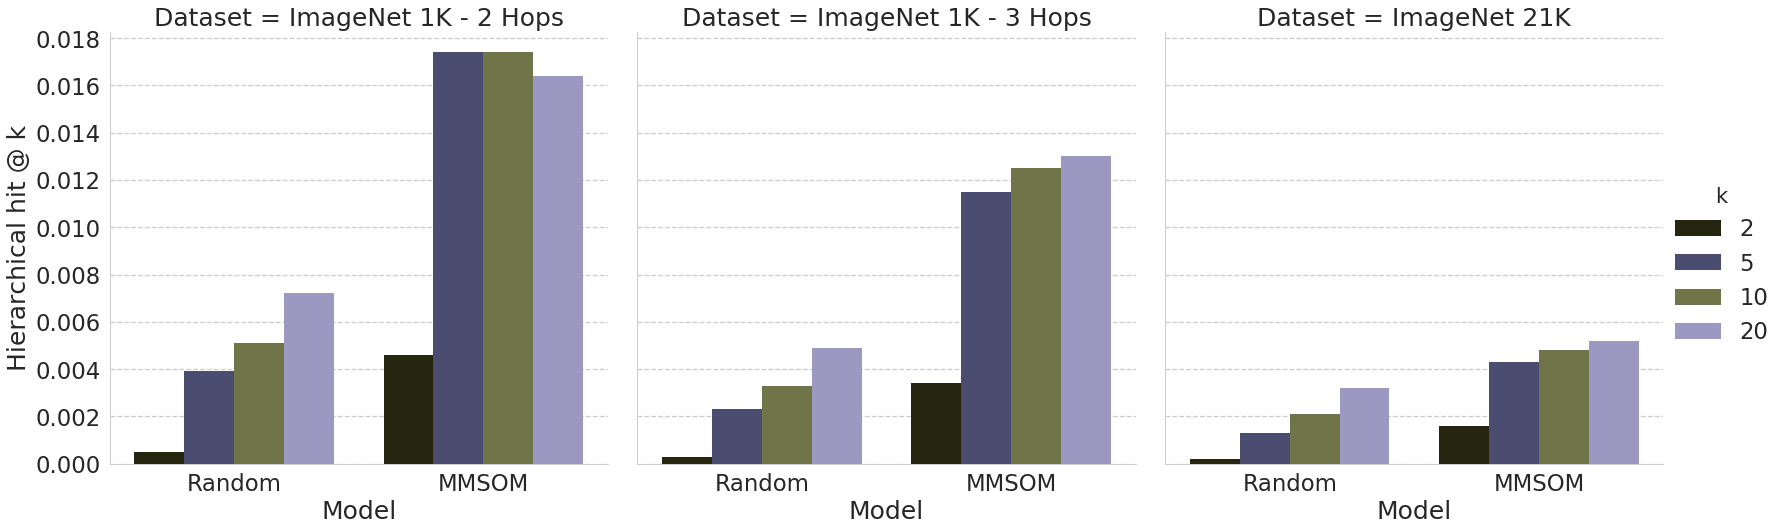
\includegraphics[width=\textwidth]{images/zero_shot_h_results.png}
    \caption{Zero-shot learning experiment - "hierarchical hit @ k" metric. The dip in performance on the \texttt{ImageNet1K - 2 Hops} dataset for the \texttt{MMSOM} model for $k=20$ w.r.t. $k=10$ and $k=5$ is due to the number of correct predictions growing slower than $k$. Before dividing by $k$, the mean number of predictions in the $CorrectSet$ were: $0.0909$, $0.1684$, $0.3244$ for $k=5$, $k=10$ and $k=20$, respectively.}
    \label{ZeroShotHierarchicalResults}
\end{figure}

\begin{table}[h]
    \centering
    \begin{footnotesize}
        \begin{tabularx}{\textwidth}{|X|c|c|c|c|c|}
            \hline
            \multirow{2}{*}{Dataset} & \multirow{2}{*}{Model}    & \multicolumn{4}{c|}{Hierarchical hit @ $k$}        \\
            \cline{3-6}              &                           & 2      & 5      & 10     & 20     \\ 
%            \hline
%            \hline
%            \multirow{2}{*}{ImageNet1K}          & Random        & 0.0031 & 0.0160 & 0.0254 & 0.0415 \\ 
%            \cline{2-6}                          & MMSOM         & 0.0171 & 0.0171 & 0.0158 & 0.0147 \\ 
            \hline
            \hline
            \multirow{2}{*}{ImageNet1K - 2 Hops} & Random        & 0.0005 & 0.0039 & 0.0051 & 0.0072 \\ 
            \cline{2-6}                          & MMSOM         & 0.0046 & 0.0174 & 0.0174 & 0.0164 \\ 
            \hline
            \hline
            \multirow{2}{*}{ImageNet1K - 3 Hops} & Random        & 0.0003 & 0.0023 & 0.0033 & 0.0049 \\ 
            \cline{2-6}                          & MMSOM         & 0.0034 & 0.0115 & 0.0125 & 0.0130 \\ 
            \hline
            \hline
            \multirow{2}{*}{ImageNet21K}         & Random        & 0.0002 & 0.0013 & 0.0021 & 0.0032 \\ 
            \cline{2-6}                          & MMSOM         & 0.0016 & 0.0043 & 0.0048 & 0.0052 \\ 
            \hline
        \end{tabularx}
    \end{footnotesize}
    \caption{Zero-shot learning experiment - "hierarchical hit @ k" metric.}
    \label{tab:ZeroShotHierarchicalResults}
\end{table}

\subsection{Analysis and interpretation of results}

Our approach out-performs the random classifier used as a baseline in all cases. This indicates that our model is indeed learning a meaningful representation of the data that goes beyond what it was originally trained to do, i.e. classification on 1000 class labels.

However, it is unclear to what extent our method is useful, given that the random classifier is one the weakest classifiers available.
An alternative baseline could have been to use the pre-trained AlexNet, but due to time constraints it was not feasible to include it in this work. It also bears mentioning that Frome et al. report better results across the board.

\end{document}